% Options for packages loaded elsewhere
\PassOptionsToPackage{unicode}{hyperref}
\PassOptionsToPackage{hyphens}{url}
\PassOptionsToPackage{dvipsnames,svgnames,x11names}{xcolor}
%
\documentclass[
  letterpaper,
  DIV=11,
  numbers=noendperiod]{scrartcl}

\usepackage{amsmath,amssymb}
\usepackage{iftex}
\ifPDFTeX
  \usepackage[T1]{fontenc}
  \usepackage[utf8]{inputenc}
  \usepackage{textcomp} % provide euro and other symbols
\else % if luatex or xetex
  \usepackage{unicode-math}
  \defaultfontfeatures{Scale=MatchLowercase}
  \defaultfontfeatures[\rmfamily]{Ligatures=TeX,Scale=1}
\fi
\usepackage{lmodern}
\ifPDFTeX\else  
    % xetex/luatex font selection
\fi
% Use upquote if available, for straight quotes in verbatim environments
\IfFileExists{upquote.sty}{\usepackage{upquote}}{}
\IfFileExists{microtype.sty}{% use microtype if available
  \usepackage[]{microtype}
  \UseMicrotypeSet[protrusion]{basicmath} % disable protrusion for tt fonts
}{}
\makeatletter
\@ifundefined{KOMAClassName}{% if non-KOMA class
  \IfFileExists{parskip.sty}{%
    \usepackage{parskip}
  }{% else
    \setlength{\parindent}{0pt}
    \setlength{\parskip}{6pt plus 2pt minus 1pt}}
}{% if KOMA class
  \KOMAoptions{parskip=half}}
\makeatother
\usepackage{xcolor}
\setlength{\emergencystretch}{3em} % prevent overfull lines
\setcounter{secnumdepth}{-\maxdimen} % remove section numbering
% Make \paragraph and \subparagraph free-standing
\ifx\paragraph\undefined\else
  \let\oldparagraph\paragraph
  \renewcommand{\paragraph}[1]{\oldparagraph{#1}\mbox{}}
\fi
\ifx\subparagraph\undefined\else
  \let\oldsubparagraph\subparagraph
  \renewcommand{\subparagraph}[1]{\oldsubparagraph{#1}\mbox{}}
\fi

\usepackage{color}
\usepackage{fancyvrb}
\newcommand{\VerbBar}{|}
\newcommand{\VERB}{\Verb[commandchars=\\\{\}]}
\DefineVerbatimEnvironment{Highlighting}{Verbatim}{commandchars=\\\{\}}
% Add ',fontsize=\small' for more characters per line
\usepackage{framed}
\definecolor{shadecolor}{RGB}{241,243,245}
\newenvironment{Shaded}{\begin{snugshade}}{\end{snugshade}}
\newcommand{\AlertTok}[1]{\textcolor[rgb]{0.68,0.00,0.00}{#1}}
\newcommand{\AnnotationTok}[1]{\textcolor[rgb]{0.37,0.37,0.37}{#1}}
\newcommand{\AttributeTok}[1]{\textcolor[rgb]{0.40,0.45,0.13}{#1}}
\newcommand{\BaseNTok}[1]{\textcolor[rgb]{0.68,0.00,0.00}{#1}}
\newcommand{\BuiltInTok}[1]{\textcolor[rgb]{0.00,0.23,0.31}{#1}}
\newcommand{\CharTok}[1]{\textcolor[rgb]{0.13,0.47,0.30}{#1}}
\newcommand{\CommentTok}[1]{\textcolor[rgb]{0.37,0.37,0.37}{#1}}
\newcommand{\CommentVarTok}[1]{\textcolor[rgb]{0.37,0.37,0.37}{\textit{#1}}}
\newcommand{\ConstantTok}[1]{\textcolor[rgb]{0.56,0.35,0.01}{#1}}
\newcommand{\ControlFlowTok}[1]{\textcolor[rgb]{0.00,0.23,0.31}{#1}}
\newcommand{\DataTypeTok}[1]{\textcolor[rgb]{0.68,0.00,0.00}{#1}}
\newcommand{\DecValTok}[1]{\textcolor[rgb]{0.68,0.00,0.00}{#1}}
\newcommand{\DocumentationTok}[1]{\textcolor[rgb]{0.37,0.37,0.37}{\textit{#1}}}
\newcommand{\ErrorTok}[1]{\textcolor[rgb]{0.68,0.00,0.00}{#1}}
\newcommand{\ExtensionTok}[1]{\textcolor[rgb]{0.00,0.23,0.31}{#1}}
\newcommand{\FloatTok}[1]{\textcolor[rgb]{0.68,0.00,0.00}{#1}}
\newcommand{\FunctionTok}[1]{\textcolor[rgb]{0.28,0.35,0.67}{#1}}
\newcommand{\ImportTok}[1]{\textcolor[rgb]{0.00,0.46,0.62}{#1}}
\newcommand{\InformationTok}[1]{\textcolor[rgb]{0.37,0.37,0.37}{#1}}
\newcommand{\KeywordTok}[1]{\textcolor[rgb]{0.00,0.23,0.31}{#1}}
\newcommand{\NormalTok}[1]{\textcolor[rgb]{0.00,0.23,0.31}{#1}}
\newcommand{\OperatorTok}[1]{\textcolor[rgb]{0.37,0.37,0.37}{#1}}
\newcommand{\OtherTok}[1]{\textcolor[rgb]{0.00,0.23,0.31}{#1}}
\newcommand{\PreprocessorTok}[1]{\textcolor[rgb]{0.68,0.00,0.00}{#1}}
\newcommand{\RegionMarkerTok}[1]{\textcolor[rgb]{0.00,0.23,0.31}{#1}}
\newcommand{\SpecialCharTok}[1]{\textcolor[rgb]{0.37,0.37,0.37}{#1}}
\newcommand{\SpecialStringTok}[1]{\textcolor[rgb]{0.13,0.47,0.30}{#1}}
\newcommand{\StringTok}[1]{\textcolor[rgb]{0.13,0.47,0.30}{#1}}
\newcommand{\VariableTok}[1]{\textcolor[rgb]{0.07,0.07,0.07}{#1}}
\newcommand{\VerbatimStringTok}[1]{\textcolor[rgb]{0.13,0.47,0.30}{#1}}
\newcommand{\WarningTok}[1]{\textcolor[rgb]{0.37,0.37,0.37}{\textit{#1}}}

\providecommand{\tightlist}{%
  \setlength{\itemsep}{0pt}\setlength{\parskip}{0pt}}\usepackage{longtable,booktabs,array}
\usepackage{calc} % for calculating minipage widths
% Correct order of tables after \paragraph or \subparagraph
\usepackage{etoolbox}
\makeatletter
\patchcmd\longtable{\par}{\if@noskipsec\mbox{}\fi\par}{}{}
\makeatother
% Allow footnotes in longtable head/foot
\IfFileExists{footnotehyper.sty}{\usepackage{footnotehyper}}{\usepackage{footnote}}
\makesavenoteenv{longtable}
\usepackage{graphicx}
\makeatletter
\def\maxwidth{\ifdim\Gin@nat@width>\linewidth\linewidth\else\Gin@nat@width\fi}
\def\maxheight{\ifdim\Gin@nat@height>\textheight\textheight\else\Gin@nat@height\fi}
\makeatother
% Scale images if necessary, so that they will not overflow the page
% margins by default, and it is still possible to overwrite the defaults
% using explicit options in \includegraphics[width, height, ...]{}
\setkeys{Gin}{width=\maxwidth,height=\maxheight,keepaspectratio}
% Set default figure placement to htbp
\makeatletter
\def\fps@figure{htbp}
\makeatother

\KOMAoption{captions}{tableheading}
\makeatletter
\@ifpackageloaded{tcolorbox}{}{\usepackage[skins,breakable]{tcolorbox}}
\@ifpackageloaded{fontawesome5}{}{\usepackage{fontawesome5}}
\definecolor{quarto-callout-color}{HTML}{909090}
\definecolor{quarto-callout-note-color}{HTML}{0758E5}
\definecolor{quarto-callout-important-color}{HTML}{CC1914}
\definecolor{quarto-callout-warning-color}{HTML}{EB9113}
\definecolor{quarto-callout-tip-color}{HTML}{00A047}
\definecolor{quarto-callout-caution-color}{HTML}{FC5300}
\definecolor{quarto-callout-color-frame}{HTML}{acacac}
\definecolor{quarto-callout-note-color-frame}{HTML}{4582ec}
\definecolor{quarto-callout-important-color-frame}{HTML}{d9534f}
\definecolor{quarto-callout-warning-color-frame}{HTML}{f0ad4e}
\definecolor{quarto-callout-tip-color-frame}{HTML}{02b875}
\definecolor{quarto-callout-caution-color-frame}{HTML}{fd7e14}
\makeatother
\makeatletter
\makeatother
\makeatletter
\makeatother
\makeatletter
\@ifpackageloaded{caption}{}{\usepackage{caption}}
\AtBeginDocument{%
\ifdefined\contentsname
  \renewcommand*\contentsname{Table of contents}
\else
  \newcommand\contentsname{Table of contents}
\fi
\ifdefined\listfigurename
  \renewcommand*\listfigurename{List of Figures}
\else
  \newcommand\listfigurename{List of Figures}
\fi
\ifdefined\listtablename
  \renewcommand*\listtablename{List of Tables}
\else
  \newcommand\listtablename{List of Tables}
\fi
\ifdefined\figurename
  \renewcommand*\figurename{Figure}
\else
  \newcommand\figurename{Figure}
\fi
\ifdefined\tablename
  \renewcommand*\tablename{Table}
\else
  \newcommand\tablename{Table}
\fi
}
\@ifpackageloaded{float}{}{\usepackage{float}}
\floatstyle{ruled}
\@ifundefined{c@chapter}{\newfloat{codelisting}{h}{lop}}{\newfloat{codelisting}{h}{lop}[chapter]}
\floatname{codelisting}{Listing}
\newcommand*\listoflistings{\listof{codelisting}{List of Listings}}
\makeatother
\makeatletter
\@ifpackageloaded{caption}{}{\usepackage{caption}}
\@ifpackageloaded{subcaption}{}{\usepackage{subcaption}}
\makeatother
\makeatletter
\@ifpackageloaded{tcolorbox}{}{\usepackage[skins,breakable]{tcolorbox}}
\makeatother
\makeatletter
\@ifundefined{shadecolor}{\definecolor{shadecolor}{rgb}{.97, .97, .97}}
\makeatother
\makeatletter
\makeatother
\makeatletter
\makeatother
\ifLuaTeX
  \usepackage{selnolig}  % disable illegal ligatures
\fi
\IfFileExists{bookmark.sty}{\usepackage{bookmark}}{\usepackage{hyperref}}
\IfFileExists{xurl.sty}{\usepackage{xurl}}{} % add URL line breaks if available
\urlstyle{same} % disable monospaced font for URLs
\hypersetup{
  pdftitle={Homework 4},
  pdfauthor={Jiaxi Li},
  colorlinks=true,
  linkcolor={blue},
  filecolor={Maroon},
  citecolor={Blue},
  urlcolor={Blue},
  pdfcreator={LaTeX via pandoc}}

\title{Homework 4}
\author{{Jiaxi Li}}
\date{}

\begin{document}
\maketitle
\ifdefined\Shaded\renewenvironment{Shaded}{\begin{tcolorbox}[frame hidden, sharp corners, interior hidden, boxrule=0pt, breakable, borderline west={3pt}{0pt}{shadecolor}, enhanced]}{\end{tcolorbox}}\fi

\renewcommand*\contentsname{Table of contents}
{
\hypersetup{linkcolor=}
\setcounter{tocdepth}{3}
\tableofcontents
}
\begin{center}\rule{0.5\linewidth}{0.5pt}\end{center}

\begin{tcolorbox}[enhanced jigsaw, leftrule=.75mm, left=2mm, coltitle=black, rightrule=.15mm, titlerule=0mm, colbacktitle=quarto-callout-important-color!10!white, toprule=.15mm, bottomrule=.15mm, opacityback=0, arc=.35mm, colframe=quarto-callout-important-color-frame, title=\textcolor{quarto-callout-important-color}{\faExclamation}\hspace{0.5em}{Important}, opacitybacktitle=0.6, toptitle=1mm, breakable, bottomtitle=1mm, colback=white]

Please read the instructions carefully before submitting your
assignment.

\begin{enumerate}
\def\labelenumi{\arabic{enumi}.}
\tightlist
\item
  This assignment requires you to only upload a \texttt{PDF} file on
  Canvas
\item
  Don't collapse any code cells before submitting.
\item
  Remember to make sure all your code output is rendered properly before
  uploading your submission.
\end{enumerate}

⚠️ Please add your name to the author information in the frontmatter
before submitting your assignment ⚠️

\end{tcolorbox}

We will be using the following libraries:

\begin{Shaded}
\begin{Highlighting}[]
\NormalTok{packages }\OtherTok{\textless{}{-}} \FunctionTok{c}\NormalTok{(}
  \StringTok{"dplyr"}\NormalTok{, }
  \StringTok{"readr"}\NormalTok{, }
  \StringTok{"tidyr"}\NormalTok{, }
  \StringTok{"purrr"}\NormalTok{, }
  \StringTok{"stringr"}\NormalTok{, }
  \StringTok{"corrplot"}\NormalTok{, }
  \StringTok{"car"}\NormalTok{, }
  \StringTok{"caret"}\NormalTok{, }
  \StringTok{"torch"}\NormalTok{, }
  \StringTok{"nnet"}\NormalTok{, }
  \StringTok{"broom"}
\NormalTok{)}

\CommentTok{\# renv::install(packages)}
\FunctionTok{sapply}\NormalTok{(packages, require, }\AttributeTok{character.only=}\NormalTok{T)}
\end{Highlighting}
\end{Shaded}

\begin{verbatim}
Loading required package: dplyr
\end{verbatim}

\begin{verbatim}

Attaching package: 'dplyr'
\end{verbatim}

\begin{verbatim}
The following objects are masked from 'package:stats':

    filter, lag
\end{verbatim}

\begin{verbatim}
The following objects are masked from 'package:base':

    intersect, setdiff, setequal, union
\end{verbatim}

\begin{verbatim}
Loading required package: readr
\end{verbatim}

\begin{verbatim}
Loading required package: tidyr
\end{verbatim}

\begin{verbatim}
Loading required package: purrr
\end{verbatim}

\begin{verbatim}
Loading required package: stringr
\end{verbatim}

\begin{verbatim}
Loading required package: corrplot
\end{verbatim}

\begin{verbatim}
corrplot 0.92 loaded
\end{verbatim}

\begin{verbatim}
Loading required package: car
\end{verbatim}

\begin{verbatim}
Loading required package: carData
\end{verbatim}

\begin{verbatim}

Attaching package: 'car'
\end{verbatim}

\begin{verbatim}
The following object is masked from 'package:purrr':

    some
\end{verbatim}

\begin{verbatim}
The following object is masked from 'package:dplyr':

    recode
\end{verbatim}

\begin{verbatim}
Loading required package: caret
\end{verbatim}

\begin{verbatim}
Warning: package 'caret' was built under R version 4.3.3
\end{verbatim}

\begin{verbatim}
Loading required package: ggplot2
\end{verbatim}

\begin{verbatim}
Loading required package: lattice
\end{verbatim}

\begin{verbatim}

Attaching package: 'caret'
\end{verbatim}

\begin{verbatim}
The following object is masked from 'package:purrr':

    lift
\end{verbatim}

\begin{verbatim}
Loading required package: torch
\end{verbatim}

\begin{verbatim}
Warning: package 'torch' was built under R version 4.3.3
\end{verbatim}

\begin{verbatim}
Loading required package: nnet
\end{verbatim}

\begin{verbatim}
Loading required package: broom
\end{verbatim}

\begin{verbatim}
   dplyr    readr    tidyr    purrr  stringr corrplot      car    caret 
    TRUE     TRUE     TRUE     TRUE     TRUE     TRUE     TRUE     TRUE 
   torch     nnet    broom 
    TRUE     TRUE     TRUE 
\end{verbatim}

\begin{center}\rule{0.5\linewidth}{0.5pt}\end{center}

\hypertarget{question-1}{%
\subsection{Question 1}\label{question-1}}

\begin{tcolorbox}[enhanced jigsaw, leftrule=.75mm, left=2mm, coltitle=black, rightrule=.15mm, titlerule=0mm, colbacktitle=quarto-callout-tip-color!10!white, toprule=.15mm, bottomrule=.15mm, opacityback=0, arc=.35mm, colframe=quarto-callout-tip-color-frame, title=\textcolor{quarto-callout-tip-color}{\faLightbulb}\hspace{0.5em}{30 points}, opacitybacktitle=0.6, toptitle=1mm, breakable, bottomtitle=1mm, colback=white]

Automatic differentiation using \texttt{torch}

\end{tcolorbox}

1.1 (5 points)

\begin{Shaded}
\begin{Highlighting}[]
\FunctionTok{library}\NormalTok{(pracma)}
\end{Highlighting}
\end{Shaded}

\begin{verbatim}
Warning: package 'pracma' was built under R version 4.3.3
\end{verbatim}

\begin{verbatim}

Attaching package: 'pracma'
\end{verbatim}

\begin{verbatim}
The following object is masked from 'package:car':

    logit
\end{verbatim}

\begin{verbatim}
The following object is masked from 'package:purrr':

    cross
\end{verbatim}

Consider \(g(x, y)\) given by

\[
g(x, y) = (x - 3)^2 + (y - 4)^2.
\]

Using elementary calculus derive the expressions for

\[
\frac{d}{dx}g(x, y), \quad \text{and} \quad \frac{d}{dy}g(x, y).
\] \# d/dx(g(x,y)) = 2x-6 d/dy(g(x,y)) = 2y-8

Using your answer from above, what is the answer to \[
\frac{d}{dx}g(x, y) \Bigg|_{(x=3, y=4)} \quad \text{and} \quad \frac{d}{dy}g(x, y) \Bigg|_{(x=3, y=4)} ?
\]

\hypertarget{ddxgx3y4-23-6-0-ddygx3y4-24-8-0}{%
\section{\texorpdfstring{d/dx(g(x=3,y=4)) = 2\emph{3-6 = 0
d/dy(g(x=3,y=4)) = 2}4-8 =
0}{d/dx(g(x=3,y=4)) = 23-6 = 0 d/dy(g(x=3,y=4)) = 24-8 = 0}}\label{ddxgx3y4-23-6-0-ddygx3y4-24-8-0}}

Define \(g(x, y)\) as a function in R, compute the gradient of
\(g(x, y)\) with respect to \(x=3\) and \(y=4\). Does the answer match
what you expected?

\begin{Shaded}
\begin{Highlighting}[]
\NormalTok{g }\OtherTok{\textless{}{-}} \ControlFlowTok{function}\NormalTok{(v) \{}
\NormalTok{  x }\OtherTok{\textless{}{-}}\NormalTok{ v[}\DecValTok{1}\NormalTok{]}
\NormalTok{  y }\OtherTok{\textless{}{-}}\NormalTok{ v[}\DecValTok{2}\NormalTok{]}
\NormalTok{  (x }\SpecialCharTok{{-}} \DecValTok{3}\NormalTok{)}\SpecialCharTok{\^{}}\DecValTok{2} \SpecialCharTok{+}\NormalTok{ (y }\SpecialCharTok{{-}} \DecValTok{4}\NormalTok{)}\SpecialCharTok{\^{}}\DecValTok{2}
\NormalTok{\}}


\NormalTok{grad\_g }\OtherTok{\textless{}{-}} \FunctionTok{grad}\NormalTok{(g, }\FunctionTok{c}\NormalTok{(}\DecValTok{3}\NormalTok{, }\DecValTok{4}\NormalTok{))}

\FunctionTok{print}\NormalTok{(grad\_g)}
\end{Highlighting}
\end{Shaded}

\begin{verbatim}
[1] 0 0
\end{verbatim}

\begin{center}\rule{0.5\linewidth}{0.5pt}\end{center}

1.2 (10 points)

\[
\newcommand{\u}{\boldsymbol{u}}\newcommand{\v}{\boldsymbol{v}}
\]

Consider \(h(\u, \v)\) given by \[
h(\u, \v) = (\u \cdot \v)^3,
\] where \(\u \cdot \v\) denotes the dot product of two vectors, i.e.,
\(\u \cdot \v = \sum_{i=1}^n u_i v_i.\)

Using elementary calculus derive the expressions for the gradients

\[
\begin{aligned}
\nabla_\u h(\u, \v) &= \Bigg(\frac{d}{du_1}h(\u, \v), \frac{d}{du_2}h(\u, \v), \dots, \frac{d}{du_n}h(\u, \v)\Bigg)
\end{aligned}
\]

Using your answer from above, what is the answer to
\(\nabla_\u h(\u, \v)\) when \(n=10\) and

\[
\begin{aligned}
\u = (-1, +1, -1, +1, -1, +1, -1, +1, -1, +1)\\
\v = (-1, -1, -1, -1, -1, +1, +1, +1, +1, +1)
\end{aligned}
\]

\hypertarget{nabla_--12-12-12-12-121212121212}{%
\section{\texorpdfstring{nabla\_\u h(\u, \v) =
(-12,-12,-12,-12,-12,12,12,12,12,12)}{nabla\_(  = (-12,-12,-12,-12,-12,12,12,12,12,12)}}\label{nabla_--12-12-12-12-121212121212}}

Define \(h(\u, \v)\) as a function in R, initialize the two vectors
\(\u\) and \(\v\) as \texttt{torch\_tensor}s. Compute the gradient of
\(h(\u, \v)\) with respect to \(\u\). Does the answer match what you
expected?

\begin{Shaded}
\begin{Highlighting}[]
\NormalTok{u }\OtherTok{\textless{}{-}} \FunctionTok{torch\_tensor}\NormalTok{(}\FunctionTok{c}\NormalTok{(}\SpecialCharTok{{-}}\DecValTok{1}\NormalTok{, }\DecValTok{1}\NormalTok{, }\SpecialCharTok{{-}}\DecValTok{1}\NormalTok{, }\DecValTok{1}\NormalTok{, }\SpecialCharTok{{-}}\DecValTok{1}\NormalTok{, }\DecValTok{1}\NormalTok{, }\SpecialCharTok{{-}}\DecValTok{1}\NormalTok{, }\DecValTok{1}\NormalTok{, }\SpecialCharTok{{-}}\DecValTok{1}\NormalTok{, }\DecValTok{1}\NormalTok{), }\AttributeTok{dtype =} \FunctionTok{torch\_float32}\NormalTok{(), }\AttributeTok{requires\_grad =} \ConstantTok{TRUE}\NormalTok{)}
\NormalTok{v }\OtherTok{\textless{}{-}} \FunctionTok{torch\_tensor}\NormalTok{(}\FunctionTok{c}\NormalTok{(}\SpecialCharTok{{-}}\DecValTok{1}\NormalTok{, }\SpecialCharTok{{-}}\DecValTok{1}\NormalTok{, }\SpecialCharTok{{-}}\DecValTok{1}\NormalTok{, }\SpecialCharTok{{-}}\DecValTok{1}\NormalTok{, }\SpecialCharTok{{-}}\DecValTok{1}\NormalTok{, }\DecValTok{1}\NormalTok{, }\DecValTok{1}\NormalTok{, }\DecValTok{1}\NormalTok{, }\DecValTok{1}\NormalTok{, }\DecValTok{1}\NormalTok{), }\AttributeTok{dtype =} \FunctionTok{torch\_float32}\NormalTok{())}
\end{Highlighting}
\end{Shaded}

\begin{Shaded}
\begin{Highlighting}[]
\NormalTok{h }\OtherTok{\textless{}{-}} \ControlFlowTok{function}\NormalTok{(u, v) \{}
\NormalTok{  (}\FunctionTok{torch\_dot}\NormalTok{(u, v))}\SpecialCharTok{\^{}}\DecValTok{3}
\NormalTok{\}}
\NormalTok{h\_value }\OtherTok{\textless{}{-}} \FunctionTok{h}\NormalTok{(u, v)}
\NormalTok{h\_value}\SpecialCharTok{$}\FunctionTok{backward}\NormalTok{()}
\NormalTok{u\_grad }\OtherTok{\textless{}{-}}\NormalTok{ u}\SpecialCharTok{$}\NormalTok{grad}
\NormalTok{u\_grad}
\end{Highlighting}
\end{Shaded}

\begin{verbatim}
torch_tensor
-12
-12
-12
-12
-12
 12
 12
 12
 12
 12
[ CPUFloatType{10} ]
\end{verbatim}

\begin{center}\rule{0.5\linewidth}{0.5pt}\end{center}

1.3 (5 points)

Consider the following function \[
f(z) = z^4 - 6z^2 - 3z + 4
\]

Derive the expression for \[
f'(z_0) = \frac{df}{dz}\Bigg|_{z=z_0}
\] and evaluate \(f'(z_0)\) when \(z_0 = -3.5\).

\hypertarget{dfdz-4z3--12z--3}{%
\section{df/dz = 4z\^{}3 -12z -3}\label{dfdz-4z3--12z--3}}

\hypertarget{fz0-3.5-4-3.52-123.5--3--132.5}{%
\section{\texorpdfstring{f'(z0=-3.5) = 4\emph{(-3.5)\^{}2 + 12}3.5 -3 =
-132.5}{f'(z0=-3.5) = 4(-3.5)\^{}2 + 123.5 -3 = -132.5}}\label{fz0-3.5-4-3.52-123.5--3--132.5}}

Define \(f(z)\) as a function in R, and using the \texttt{torch} library
compute \(f'(-3.5)\).

\begin{Shaded}
\begin{Highlighting}[]
\NormalTok{f }\OtherTok{\textless{}{-}} \ControlFlowTok{function}\NormalTok{(z) \{}
\NormalTok{  z}\SpecialCharTok{\^{}}\DecValTok{4} \SpecialCharTok{{-}} \DecValTok{6}\SpecialCharTok{*}\NormalTok{z}\SpecialCharTok{\^{}}\DecValTok{2} \SpecialCharTok{{-}} \DecValTok{3}\SpecialCharTok{*}\NormalTok{z }\SpecialCharTok{+} \DecValTok{4}
\NormalTok{\}}


\NormalTok{df\_dz }\OtherTok{\textless{}{-}} \ControlFlowTok{function}\NormalTok{(z) \{}
  \DecValTok{4}\SpecialCharTok{*}\NormalTok{z}\SpecialCharTok{\^{}}\DecValTok{3} \SpecialCharTok{{-}} \DecValTok{12}\SpecialCharTok{*}\NormalTok{z }\SpecialCharTok{{-}} \DecValTok{3}
\NormalTok{\}}


\NormalTok{df\_dz\_at\_z0 }\OtherTok{\textless{}{-}} \FunctionTok{df\_dz}\NormalTok{(}\SpecialCharTok{{-}}\FloatTok{3.5}\NormalTok{)}
\NormalTok{df\_dz\_at\_z0}
\end{Highlighting}
\end{Shaded}

\begin{verbatim}
[1] -132.5
\end{verbatim}

\begin{center}\rule{0.5\linewidth}{0.5pt}\end{center}

1.4 (5 points)

For the same function \(f\), initialize \(z[1] = -3.5\), and perform
\(n=100\) iterations of \textbf{gradient descent}, i.e.,

\begin{quote}
\(z[{k+1}] = z[k] - \eta f'(z[k]) \ \ \ \ \) for
\(k = 1, 2, \dots, 100\)
\end{quote}

Plot the curve \(f\) and add taking \(\eta = 0.02\), add the points
\(\{z_0, z_1, z_2, \dots z_{100}\}\) obtained using gradient descent to
the plot. What do you observe?

\begin{Shaded}
\begin{Highlighting}[]
\NormalTok{z }\OtherTok{\textless{}{-}} \SpecialCharTok{{-}}\FloatTok{3.5}
\NormalTok{eta\_1 }\OtherTok{\textless{}{-}} \FloatTok{0.02}
\NormalTok{n\_iterations }\OtherTok{\textless{}{-}} \DecValTok{100}

\NormalTok{gradient\_descent }\OtherTok{\textless{}{-}} \ControlFlowTok{function}\NormalTok{(initial\_value, learning\_rate, n\_iterations, derivative\_func) \{}
\NormalTok{  z }\OtherTok{\textless{}{-}}\NormalTok{ initial\_value}
\NormalTok{  z\_history }\OtherTok{\textless{}{-}} \FunctionTok{numeric}\NormalTok{(n\_iterations)}
  \ControlFlowTok{for}\NormalTok{ (i }\ControlFlowTok{in} \DecValTok{1}\SpecialCharTok{:}\NormalTok{n\_iterations) \{}
\NormalTok{    z }\OtherTok{\textless{}{-}}\NormalTok{ z }\SpecialCharTok{{-}}\NormalTok{ learning\_rate }\SpecialCharTok{*} \FunctionTok{derivative\_func}\NormalTok{(z)}
\NormalTok{    z\_history[i] }\OtherTok{\textless{}{-}}\NormalTok{ z}
\NormalTok{  \}}
\NormalTok{  z\_history}
\NormalTok{\}}

\NormalTok{z\_history\_1 }\OtherTok{\textless{}{-}} \FunctionTok{gradient\_descent}\NormalTok{(z, eta\_1, n\_iterations, df\_dz)}
\end{Highlighting}
\end{Shaded}

\begin{Shaded}
\begin{Highlighting}[]
\FunctionTok{plot}\NormalTok{(}\DecValTok{1}\SpecialCharTok{:}\NormalTok{n\_iterations, z\_history\_1,  }\AttributeTok{col =} \StringTok{\textquotesingle{}blue\textquotesingle{}}\NormalTok{, }\AttributeTok{ylim =} \FunctionTok{range}\NormalTok{(z\_history\_1), }\AttributeTok{ylab =} \StringTok{\textquotesingle{}z value\textquotesingle{}}\NormalTok{, }\AttributeTok{xlab =} \StringTok{\textquotesingle{}Iteration\textquotesingle{}}\NormalTok{, }\AttributeTok{main =} \StringTok{\textquotesingle{}Gradient Descent Progress\textquotesingle{}}\NormalTok{)}
\end{Highlighting}
\end{Shaded}

\begin{figure}[H]

{\centering 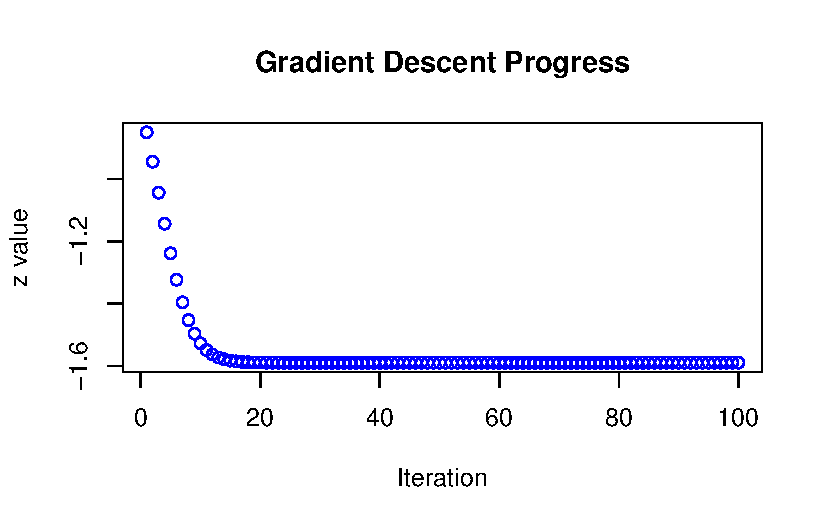
\includegraphics{hm4_files/figure-pdf/unnamed-chunk-8-1.pdf}

}

\end{figure}

\begin{Shaded}
\begin{Highlighting}[]
\NormalTok{legend}\OtherTok{=}\FunctionTok{c}\NormalTok{(}\StringTok{"eta = 0.02"}\NormalTok{)}
\end{Highlighting}
\end{Shaded}

\begin{center}\rule{0.5\linewidth}{0.5pt}\end{center}

1.5 (5 points)

Redo the same analysis as \textbf{Question 1.4}, but this time using
\(\eta = 0.03\). What do you observe? What can you conclude from this
analysis

\begin{Shaded}
\begin{Highlighting}[]
\NormalTok{eta\_2 }\OtherTok{\textless{}{-}} \FloatTok{0.03}
\NormalTok{z\_history\_2 }\OtherTok{\textless{}{-}} \FunctionTok{gradient\_descent}\NormalTok{(z, eta\_2, n\_iterations, df\_dz)}

\FunctionTok{plot}\NormalTok{(}\DecValTok{1}\SpecialCharTok{:}\NormalTok{n\_iterations, z\_history\_1, }\AttributeTok{type =} \StringTok{\textquotesingle{}l\textquotesingle{}}\NormalTok{, }\AttributeTok{col =} \StringTok{\textquotesingle{}blue\textquotesingle{}}\NormalTok{, }\AttributeTok{ylim =} \FunctionTok{range}\NormalTok{(}\FunctionTok{c}\NormalTok{(z\_history\_1, z\_history\_2)), }\AttributeTok{ylab =} \StringTok{\textquotesingle{}z value\textquotesingle{}}\NormalTok{, }\AttributeTok{xlab =} \StringTok{\textquotesingle{}Iteration\textquotesingle{}}\NormalTok{, }\AttributeTok{main =} \StringTok{\textquotesingle{}Gradient Descent Progress\textquotesingle{}}\NormalTok{)}
\FunctionTok{lines}\NormalTok{(}\DecValTok{1}\SpecialCharTok{:}\NormalTok{n\_iterations, z\_history\_2, }\AttributeTok{col =} \StringTok{\textquotesingle{}red\textquotesingle{}}\NormalTok{)}
\FunctionTok{legend}\NormalTok{(}\StringTok{"topright"}\NormalTok{, }\AttributeTok{legend=}\FunctionTok{c}\NormalTok{(}\StringTok{"eta = 0.02"}\NormalTok{, }\StringTok{"eta = 0.03"}\NormalTok{), }\AttributeTok{col=}\FunctionTok{c}\NormalTok{(}\StringTok{"blue"}\NormalTok{, }\StringTok{"red"}\NormalTok{), }\AttributeTok{lty=}\DecValTok{1}\SpecialCharTok{:}\DecValTok{1}\NormalTok{)}
\end{Highlighting}
\end{Shaded}

\begin{figure}[H]

{\centering 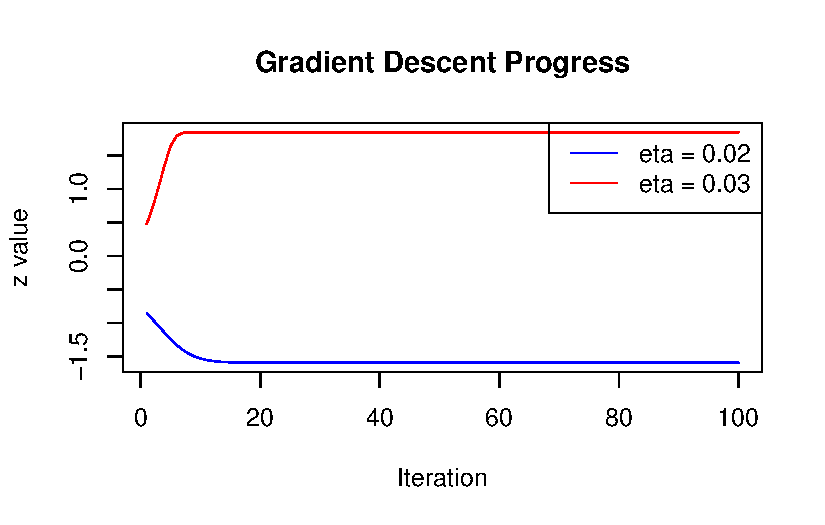
\includegraphics{hm4_files/figure-pdf/unnamed-chunk-9-1.pdf}

}

\end{figure}

\hypertarget{during-the-iteration-increas-the-0.03-of-it-z-value-increase-but-0.02-z-valuewas-going-down}{%
\section{\texorpdfstring{during the iteration increas the \eta = 0.03 of
it z value increase, but \eta = 0.02 z valuewas going
down}{during the iteration increas the = 0.03 of it z value increase, but = 0.02 z valuewas going down}}\label{during-the-iteration-increas-the-0.03-of-it-z-value-increase-but-0.02-z-valuewas-going-down}}

\hypertarget{but-they-all-finally-approach-a-steaady-value-like-0.02-stick-in--1.5-and-0.03-stick-in-1.5}{%
\section{but they all finally approach a steaady value like 0.02 stick
in -1.5 and 0.03 stick in
1.5}\label{but-they-all-finally-approach-a-steaady-value-like-0.02-stick-in--1.5-and-0.03-stick-in-1.5}}

\hypertarget{the-choice-of-learning-rate-is-crucial-for-the-performance-of-gradient-descent}{%
\section{The choice of learning rate is crucial for the performance of
gradient
descent}\label{the-choice-of-learning-rate-is-crucial-for-the-performance-of-gradient-descent}}

\begin{center}\rule{0.5\linewidth}{0.5pt}\end{center}

\hypertarget{question-2}{%
\subsection{Question 2}\label{question-2}}

\begin{tcolorbox}[enhanced jigsaw, leftrule=.75mm, left=2mm, coltitle=black, rightrule=.15mm, titlerule=0mm, colbacktitle=quarto-callout-tip-color!10!white, toprule=.15mm, bottomrule=.15mm, opacityback=0, arc=.35mm, colframe=quarto-callout-tip-color-frame, title=\textcolor{quarto-callout-tip-color}{\faLightbulb}\hspace{0.5em}{50 points}, opacitybacktitle=0.6, toptitle=1mm, breakable, bottomtitle=1mm, colback=white]

Logistic regression and interpretation of effect sizes

\end{tcolorbox}

For this question we will use the \textbf{Titanic} dataset from the
Stanford data archive. This dataset contains information about
passengers aboard the Titanic and whether or not they survived.

\begin{center}\rule{0.5\linewidth}{0.5pt}\end{center}

2.1 (5 points)

Read the data from the following URL as a tibble in R. Preprocess the
data such that the variables are of the right data type, e.g., binary
variables are encoded as factors, and convert all column names to lower
case for consistency. Let's also rename the response variable
\texttt{Survival} to \texttt{y} for convenience.

\begin{Shaded}
\begin{Highlighting}[]
\NormalTok{url }\OtherTok{\textless{}{-}} \StringTok{"https://web.stanford.edu/class/archive/cs/cs109/cs109.1166/stuff/titanic.csv"}

\NormalTok{df }\OtherTok{\textless{}{-}} \FunctionTok{read\_csv}\NormalTok{(url) }\CommentTok{\# Insert your code here}
\end{Highlighting}
\end{Shaded}

\begin{verbatim}
Rows: 887 Columns: 8
-- Column specification --------------------------------------------------------
Delimiter: ","
chr (2): Name, Sex
dbl (6): Survived, Pclass, Age, Siblings/Spouses Aboard, Parents/Children Ab...

i Use `spec()` to retrieve the full column specification for this data.
i Specify the column types or set `show_col_types = FALSE` to quiet this message.
\end{verbatim}

\begin{Shaded}
\begin{Highlighting}[]
\NormalTok{titanic\_data }\OtherTok{\textless{}{-}}\NormalTok{ df }\SpecialCharTok{\%\textgreater{}\%}
  \FunctionTok{mutate}\NormalTok{(}\FunctionTok{across}\NormalTok{(}\FunctionTok{where}\NormalTok{(is.character), as.factor)) }\SpecialCharTok{\%\textgreater{}\%} 
  \FunctionTok{rename\_with}\NormalTok{(tolower, }\FunctionTok{everything}\NormalTok{()) }\SpecialCharTok{\%\textgreater{}\%}
  \FunctionTok{rename}\NormalTok{(}\AttributeTok{y =}\NormalTok{ survived)}


\FunctionTok{head}\NormalTok{(titanic\_data)}
\end{Highlighting}
\end{Shaded}

\begin{verbatim}
# A tibble: 6 x 8
      y pclass name    sex     age siblings/spouses abo~1 parents/children abo~2
  <dbl>  <dbl> <fct>   <fct> <dbl>                  <dbl>                  <dbl>
1     0      3 Mr. Ow~ male     22                      1                      0
2     1      1 Mrs. J~ fema~    38                      1                      0
3     1      3 Miss. ~ fema~    26                      0                      0
4     1      1 Mrs. J~ fema~    35                      1                      0
5     0      3 Mr. Wi~ male     35                      0                      0
6     0      3 Mr. Ja~ male     27                      0                      0
# i abbreviated names: 1: `siblings/spouses aboard`,
#   2: `parents/children aboard`
# i 1 more variable: fare <dbl>
\end{verbatim}

\begin{center}\rule{0.5\linewidth}{0.5pt}\end{center}

2.2 (5 points)

Visualize the correlation matrix of all numeric columns in \texttt{df}
using \texttt{corrplot()}

\begin{Shaded}
\begin{Highlighting}[]
\NormalTok{numeric\_columns }\OtherTok{\textless{}{-}}\NormalTok{ titanic\_data }\SpecialCharTok{\%\textgreater{}\%} \FunctionTok{select}\NormalTok{(}\FunctionTok{where}\NormalTok{(is.numeric))}
\NormalTok{cor\_matrix }\OtherTok{\textless{}{-}} \FunctionTok{cor}\NormalTok{(numeric\_columns)}
\FunctionTok{corrplot}\NormalTok{(cor\_matrix, }\AttributeTok{method =} \StringTok{"circle"}\NormalTok{)}
\end{Highlighting}
\end{Shaded}

\begin{figure}[H]

{\centering 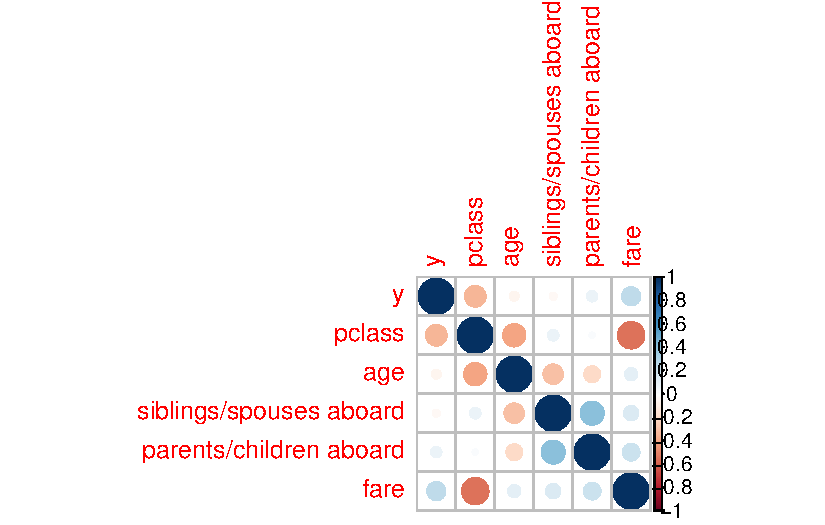
\includegraphics{hm4_files/figure-pdf/unnamed-chunk-11-1.pdf}

}

\end{figure}

\begin{center}\rule{0.5\linewidth}{0.5pt}\end{center}

2.3 (10 points)

Fit a logistic regression model to predict the probability of surviving
the titanic as a function of:

\begin{itemize}
\tightlist
\item
  \texttt{pclass}
\item
  \texttt{sex}
\item
  \texttt{age}
\item
  \texttt{fare}
\item
  \texttt{\#\ siblings}
\item
  \texttt{\#\ parents}
\end{itemize}

\begin{Shaded}
\begin{Highlighting}[]
\FunctionTok{names}\NormalTok{(titanic\_data) }\OtherTok{\textless{}{-}} \FunctionTok{gsub}\NormalTok{(}\StringTok{" "}\NormalTok{, }\StringTok{"\_"}\NormalTok{, }\FunctionTok{names}\NormalTok{(titanic\_data))}
\NormalTok{titanic\_data }\OtherTok{\textless{}{-}}\NormalTok{ titanic\_data }\SpecialCharTok{\%\textgreater{}\%}
  \FunctionTok{rename}\NormalTok{(}\AttributeTok{siblings =} \StringTok{\textasciigrave{}}\AttributeTok{siblings/spouses\_aboard}\StringTok{\textasciigrave{}}\NormalTok{, }\AttributeTok{parents =} \StringTok{\textasciigrave{}}\AttributeTok{parents/children\_aboard}\StringTok{\textasciigrave{}}\NormalTok{)}
\end{Highlighting}
\end{Shaded}

\begin{Shaded}
\begin{Highlighting}[]
\NormalTok{full\_model }\OtherTok{\textless{}{-}} \FunctionTok{glm}\NormalTok{(y }\SpecialCharTok{\textasciitilde{}}\NormalTok{ pclass }\SpecialCharTok{+}\NormalTok{ sex }\SpecialCharTok{+}\NormalTok{ age }\SpecialCharTok{+}\NormalTok{ fare }\SpecialCharTok{+}\NormalTok{ siblings }\SpecialCharTok{+}\NormalTok{ parents, }
                  \AttributeTok{data =}\NormalTok{ titanic\_data) }\CommentTok{\# Insert your code here}
\FunctionTok{summary}\NormalTok{(full\_model)}
\end{Highlighting}
\end{Shaded}

\begin{verbatim}

Call:
glm(formula = y ~ pclass + sex + age + fare + siblings + parents, 
    data = titanic_data)

Coefficients:
              Estimate Std. Error t value Pr(>|t|)    
(Intercept)  1.3320583  0.0711052  18.734  < 2e-16 ***
pclass      -0.1800338  0.0200993  -8.957  < 2e-16 ***
sexmale     -0.5077356  0.0279609 -18.159  < 2e-16 ***
age         -0.0061972  0.0010359  -5.983 3.19e-09 ***
fare         0.0004034  0.0003230   1.249 0.212020    
siblings    -0.0502913  0.0131963  -3.811 0.000148 ***
parents     -0.0192834  0.0180771  -1.067 0.286387    
---
Signif. codes:  0 '***' 0.001 '**' 0.01 '*' 0.05 '.' 0.1 ' ' 1

(Dispersion parameter for gaussian family taken to be 0.1438727)

    Null deviance: 210.14  on 886  degrees of freedom
Residual deviance: 126.61  on 880  degrees of freedom
AIC: 806.43

Number of Fisher Scoring iterations: 2
\end{verbatim}

\begin{center}\rule{0.5\linewidth}{0.5pt}\end{center}

2.4 (30 points)

Provide an interpretation for the slope and intercept terms estimated in
\texttt{full\_model} in terms of the log-odds of survival in the titanic
and in terms of the odds-ratio (if the covariate is also categorical).

\hypertarget{section}{%
\subsection{}\label{section}}

Recall the definition of logistic regression from the lecture notes, and
also recall how we interpreted the slope in the linear regression model
(particularly when the covariate was categorical).

\hypertarget{from-estimate-and-interpret-the-significant-predictors-of-survival-on-the-titanic-in-this-model-are-the-passenger-class-gender-age-and-the-number-of-siblingsspouses-aboard-with-class-and-gender-having-the-most-substantial-effects.-the-fare-and-number-of-parentschildren-do-not-seem-to-have-a-significant-impact-when-controlling-for-other-factors.}{%
\section{from Estimate and interpret the significant predictors of
survival on the Titanic in this model are the passenger class, gender,
age, and the number of siblings/spouses aboard, with class and gender
having the most substantial effects. The fare and number of
parents/children do not seem to have a significant impact when
controlling for other
factors.}\label{from-estimate-and-interpret-the-significant-predictors-of-survival-on-the-titanic-in-this-model-are-the-passenger-class-gender-age-and-the-number-of-siblingsspouses-aboard-with-class-and-gender-having-the-most-substantial-effects.-the-fare-and-number-of-parentschildren-do-not-seem-to-have-a-significant-impact-when-controlling-for-other-factors.}}

\begin{center}\rule{0.5\linewidth}{0.5pt}\end{center}

\hypertarget{question-3}{%
\subsection{Question 3}\label{question-3}}

\begin{tcolorbox}[enhanced jigsaw, leftrule=.75mm, left=2mm, coltitle=black, rightrule=.15mm, titlerule=0mm, colbacktitle=quarto-callout-tip-color!10!white, toprule=.15mm, bottomrule=.15mm, opacityback=0, arc=.35mm, colframe=quarto-callout-tip-color-frame, title=\textcolor{quarto-callout-tip-color}{\faLightbulb}\hspace{0.5em}{70 points}, opacitybacktitle=0.6, toptitle=1mm, breakable, bottomtitle=1mm, colback=white]

Variable selection and logistic regression in \texttt{torch}

\end{tcolorbox}

\begin{center}\rule{0.5\linewidth}{0.5pt}\end{center}

3.1 (15 points)

Complete the following function \texttt{overview} which takes in two
categorical vectors (\texttt{predicted} and \texttt{expected}) and
outputs:

\begin{itemize}
\tightlist
\item
  The prediction accuracy
\item
  The prediction error
\item
  The false positive rate, and
\item
  The false negative rate
\end{itemize}

\begin{Shaded}
\begin{Highlighting}[]
\NormalTok{overview }\OtherTok{\textless{}{-}} \ControlFlowTok{function}\NormalTok{(predicted, expected)\{}
\NormalTok{    accuracy }\OtherTok{\textless{}{-}} \FunctionTok{sum}\NormalTok{(predicted }\SpecialCharTok{==}\NormalTok{ expected) }\SpecialCharTok{/} \FunctionTok{length}\NormalTok{(expected) }\CommentTok{\# Insert your code here}
\NormalTok{    error }\OtherTok{\textless{}{-}} \DecValTok{1} \SpecialCharTok{{-}}\NormalTok{ accuracy }\CommentTok{\# Insert your code here}
\NormalTok{    total\_false\_positives }\OtherTok{\textless{}{-}} \FunctionTok{sum}\NormalTok{((predicted }\SpecialCharTok{==} \DecValTok{1}\NormalTok{) }\SpecialCharTok{\&}\NormalTok{ (expected }\SpecialCharTok{==} \DecValTok{0}\NormalTok{)) }\CommentTok{\# Insert your code here}
\NormalTok{    total\_true\_positives }\OtherTok{\textless{}{-}} \FunctionTok{sum}\NormalTok{((predicted }\SpecialCharTok{==} \DecValTok{1}\NormalTok{) }\SpecialCharTok{\&}\NormalTok{ (expected }\SpecialCharTok{==} \DecValTok{1}\NormalTok{)) }\CommentTok{\# Insert your code here}
\NormalTok{    total\_false\_negatives }\OtherTok{\textless{}{-}} \FunctionTok{sum}\NormalTok{((predicted }\SpecialCharTok{==} \DecValTok{0}\NormalTok{) }\SpecialCharTok{\&}\NormalTok{ (expected }\SpecialCharTok{==} \DecValTok{1}\NormalTok{)) }\CommentTok{\# Insert your code here}
\NormalTok{    total\_true\_negatives }\OtherTok{\textless{}{-}} \FunctionTok{sum}\NormalTok{((predicted }\SpecialCharTok{==} \DecValTok{0}\NormalTok{) }\SpecialCharTok{\&}\NormalTok{ (expected }\SpecialCharTok{==} \DecValTok{0}\NormalTok{)) }\CommentTok{\# Insert your code here}
\NormalTok{    false\_positive\_rate }\OtherTok{\textless{}{-}}\NormalTok{ total\_false\_positives}\SpecialCharTok{/}\FunctionTok{length}\NormalTok{(expected) }\CommentTok{\# Insert your code here}
\NormalTok{    false\_negative\_rate }\OtherTok{\textless{}{-}}\NormalTok{ total\_false\_negatives}\SpecialCharTok{/}\FunctionTok{length}\NormalTok{(expected) }\CommentTok{\# Insert your code here}
    \FunctionTok{return}\NormalTok{(}
        \FunctionTok{data.frame}\NormalTok{(}
            \AttributeTok{accuracy =}\NormalTok{ accuracy, }
            \AttributeTok{error=}\NormalTok{error, }
            \AttributeTok{false\_positive\_rate =}\NormalTok{ false\_positive\_rate, }
            \AttributeTok{false\_negative\_rate =}\NormalTok{ false\_negative\_rate}
\NormalTok{        )}
\NormalTok{    )}
\NormalTok{\}}
\end{Highlighting}
\end{Shaded}

You can check if your function is doing what it's supposed to do by
evaluating

\begin{Shaded}
\begin{Highlighting}[]
\FunctionTok{overview}\NormalTok{(titanic\_data}\SpecialCharTok{$}\NormalTok{y, titanic\_data}\SpecialCharTok{$}\NormalTok{y)}
\end{Highlighting}
\end{Shaded}

\begin{verbatim}
  accuracy error false_positive_rate false_negative_rate
1        1     0                   0                   0
\end{verbatim}

and making sure that the accuracy is \(100\%\) while the errors are
\(0\%\).

\begin{center}\rule{0.5\linewidth}{0.5pt}\end{center}

3.2 (5 points)

Display an overview of the key performance metrics of
\texttt{full\_model}

\begin{Shaded}
\begin{Highlighting}[]
\FunctionTok{overview}\NormalTok{(full\_model}\SpecialCharTok{$}\NormalTok{data, titanic\_data}\SpecialCharTok{$}\NormalTok{y)}
\end{Highlighting}
\end{Shaded}

\begin{verbatim}
  accuracy     error false_positive_rate false_negative_rate
1 2.315671 -1.315671           0.2615558           0.5005637
\end{verbatim}

\begin{center}\rule{0.5\linewidth}{0.5pt}\end{center}

3.3 (5 points)

Using backward-stepwise logistic regression, find a parsimonious
altenative to \texttt{full\_model}, and print its \texttt{overview}

\begin{Shaded}
\begin{Highlighting}[]
\NormalTok{step\_model }\OtherTok{\textless{}{-}} \FunctionTok{step}\NormalTok{(full\_model, }\AttributeTok{direction=}\StringTok{"backward"}\NormalTok{) }\CommentTok{\# Insert your code here. }
\end{Highlighting}
\end{Shaded}

\begin{verbatim}
Start:  AIC=806.43
y ~ pclass + sex + age + fare + siblings + parents

           Df Deviance     AIC
- parents   1   126.77  805.58
- fare      1   126.83  806.00
<none>          126.61  806.43
- siblings  1   128.70  818.95
- age       1   131.76  839.79
- pclass    1   138.15  881.82
- sex       1   174.05 1086.71

Step:  AIC=805.58
y ~ pclass + sex + age + fare + siblings

           Df Deviance     AIC
- fare      1   126.94  804.76
<none>          126.77  805.58
- siblings  1   129.60  823.15
- age       1   131.83  838.27
- pclass    1   138.62  882.82
- sex       1   174.96 1089.35

Step:  AIC=804.76
y ~ pclass + sex + age + siblings

           Df Deviance     AIC
<none>          126.94  804.76
- siblings  1   129.60  821.17
- age       1   132.11  838.19
- pclass    1   145.96  926.61
- sex       1   176.17 1093.45
\end{verbatim}

\begin{Shaded}
\begin{Highlighting}[]
\FunctionTok{summary}\NormalTok{(step\_model)}
\end{Highlighting}
\end{Shaded}

\begin{verbatim}

Call:
glm(formula = y ~ pclass + sex + age + siblings, data = titanic_data)

Coefficients:
             Estimate Std. Error t value Pr(>|t|)    
(Intercept)  1.367793   0.060360  22.661  < 2e-16 ***
pclass      -0.193543   0.016835 -11.496  < 2e-16 ***
sexmale     -0.504846   0.027297 -18.495  < 2e-16 ***
age         -0.006191   0.001033  -5.995 2.96e-09 ***
siblings    -0.052207   0.012138  -4.301 1.89e-05 ***
---
Signif. codes:  0 '***' 0.001 '**' 0.01 '*' 0.05 '.' 0.1 ' ' 1

(Dispersion parameter for gaussian family taken to be 0.1439234)

    Null deviance: 210.14  on 886  degrees of freedom
Residual deviance: 126.94  on 882  degrees of freedom
AIC: 804.76

Number of Fisher Scoring iterations: 2
\end{verbatim}

\begin{Shaded}
\begin{Highlighting}[]
\NormalTok{step\_predictions }\OtherTok{\textless{}{-}} \FunctionTok{predict}\NormalTok{(step\_model, }\AttributeTok{type =} \StringTok{"response"}\NormalTok{) }\CommentTok{\# Insert your code here}
\FunctionTok{overview}\NormalTok{(step\_predictions, titanic\_data}\SpecialCharTok{$}\NormalTok{y)}
\end{Highlighting}
\end{Shaded}

\begin{verbatim}
  accuracy error false_positive_rate false_negative_rate
1        0     1                   0                   0
\end{verbatim}

\begin{center}\rule{0.5\linewidth}{0.5pt}\end{center}

3.4 (15 points)

Using the \texttt{caret} package, setup a \textbf{\(5\)-fold
cross-validation} training method using the
\texttt{caret::trainConrol()} function

\begin{Shaded}
\begin{Highlighting}[]
\NormalTok{controls }\OtherTok{\textless{}{-}} \FunctionTok{trainControl}\NormalTok{(}\AttributeTok{method=}\StringTok{"cv"}\NormalTok{, }\AttributeTok{number=}\DecValTok{5}\NormalTok{) }\CommentTok{\# ... insert your code here}
\end{Highlighting}
\end{Shaded}

Now, using \texttt{control}, perform \(5\)-fold cross validation using
\texttt{caret::train()} to select the optimal \(\lambda\) parameter for
LASSO with logistic regression.

Take the search grid for \(\lambda\) to be in
\(\{ 2^{-20}, 2^{-19.5}, 2^{-19}, \dots, 2^{-0.5}, 2^{0} \}\).

\begin{Shaded}
\begin{Highlighting}[]
\CommentTok{\# Insert your code in the ... region}
\NormalTok{lasso\_fit }\OtherTok{\textless{}{-}} \FunctionTok{train}\NormalTok{(}
  \AttributeTok{x =}\NormalTok{ titanic\_data[, }\SpecialCharTok{{-}}\FunctionTok{which}\NormalTok{(}\FunctionTok{names}\NormalTok{(titanic\_data) }\SpecialCharTok{==} \StringTok{"y"}\NormalTok{)],}
  \AttributeTok{y =}\NormalTok{ titanic\_data}\SpecialCharTok{$}\NormalTok{y,}
  \AttributeTok{method =} \StringTok{"glmnet"}\NormalTok{,}
  \AttributeTok{trControl =}\NormalTok{ controls, }
  \AttributeTok{tuneGrid =} \FunctionTok{expand.grid}\NormalTok{(}
    \AttributeTok{alpha =} \DecValTok{1}\NormalTok{,}
    \AttributeTok{lambda =} \DecValTok{2}\SpecialCharTok{\^{}}\FunctionTok{seq}\NormalTok{(}\SpecialCharTok{{-}}\DecValTok{20}\NormalTok{, }\DecValTok{0}\NormalTok{, }\AttributeTok{by =} \FloatTok{0.5}\NormalTok{)}
\NormalTok{    ),}
  \AttributeTok{family =} \StringTok{"binomial"}
\NormalTok{)}
\end{Highlighting}
\end{Shaded}

\begin{verbatim}
Warning in train.default(x = titanic_data[, -which(names(titanic_data) == : You
are trying to do regression and your outcome only has two possible values Are
you trying to do classification? If so, use a 2 level factor as your outcome
column.
\end{verbatim}

\begin{verbatim}
Warning: Setting row names on a tibble is deprecated.
\end{verbatim}

\begin{verbatim}
Warning in storage.mode(xd) <- "double": NAs introduced by coercion
\end{verbatim}

\begin{verbatim}
Warning in cbind2(1, newx) %*% nbeta: NAs introduced by coercion

Warning in cbind2(1, newx) %*% nbeta: NAs introduced by coercion
\end{verbatim}

\begin{verbatim}
Warning: Setting row names on a tibble is deprecated.
\end{verbatim}

\begin{verbatim}
Warning in storage.mode(xd) <- "double": NAs introduced by coercion
\end{verbatim}

\begin{verbatim}
Warning in cbind2(1, newx) %*% nbeta: NAs introduced by coercion

Warning in cbind2(1, newx) %*% nbeta: NAs introduced by coercion
\end{verbatim}

\begin{verbatim}
Warning: Setting row names on a tibble is deprecated.
\end{verbatim}

\begin{verbatim}
Warning in storage.mode(xd) <- "double": NAs introduced by coercion
\end{verbatim}

\begin{verbatim}
Warning in cbind2(1, newx) %*% nbeta: NAs introduced by coercion

Warning in cbind2(1, newx) %*% nbeta: NAs introduced by coercion
\end{verbatim}

\begin{verbatim}
Warning: Setting row names on a tibble is deprecated.
\end{verbatim}

\begin{verbatim}
Warning in storage.mode(xd) <- "double": NAs introduced by coercion
\end{verbatim}

\begin{verbatim}
Warning in cbind2(1, newx) %*% nbeta: NAs introduced by coercion

Warning in cbind2(1, newx) %*% nbeta: NAs introduced by coercion
\end{verbatim}

\begin{verbatim}
Warning: Setting row names on a tibble is deprecated.
\end{verbatim}

\begin{verbatim}
Warning in storage.mode(xd) <- "double": NAs introduced by coercion
\end{verbatim}

\begin{verbatim}
Warning in cbind2(1, newx) %*% nbeta: NAs introduced by coercion

Warning in cbind2(1, newx) %*% nbeta: NAs introduced by coercion
\end{verbatim}

\begin{verbatim}
Warning in nominalTrainWorkflow(x = x, y = y, wts = weights, info = trainInfo,
: There were missing values in resampled performance measures.
\end{verbatim}

\begin{verbatim}
Warning: Setting row names on a tibble is deprecated.
\end{verbatim}

\begin{verbatim}
Warning in storage.mode(xd) <- "double": NAs introduced by coercion
\end{verbatim}

\begin{Shaded}
\begin{Highlighting}[]
\FunctionTok{print}\NormalTok{(lasso\_fit)}
\end{Highlighting}
\end{Shaded}

\begin{verbatim}
glmnet 

887 samples
  7 predictor

No pre-processing
Resampling: Cross-Validated (5 fold) 
Summary of sample sizes: 710, 710, 709, 709, 710 
Resampling results across tuning parameters:

  lambda        RMSE       Rsquared    MAE      
  9.536743e-07  1.2765642  0.16662435  1.0883331
  1.348699e-06  1.2765642  0.16662435  1.0883331
  1.907349e-06  1.2765642  0.16662435  1.0883331
  2.697398e-06  1.2765642  0.16662435  1.0883331
  3.814697e-06  1.2765642  0.16662435  1.0883331
  5.394797e-06  1.2765642  0.16662435  1.0883331
  7.629395e-06  1.2765642  0.16662435  1.0883331
  1.078959e-05  1.2765642  0.16662435  1.0883331
  1.525879e-05  1.2765642  0.16662435  1.0883331
  2.157919e-05  1.2765642  0.16662435  1.0883331
  3.051758e-05  1.2765642  0.16662435  1.0883331
  4.315837e-05  1.2765642  0.16662435  1.0883331
  6.103516e-05  1.2765642  0.16662435  1.0883331
  8.631675e-05  1.2765642  0.16662435  1.0883331
  1.220703e-04  1.2765642  0.16662435  1.0883331
  1.726335e-04  1.2765642  0.16662435  1.0883331
  2.441406e-04  1.2765642  0.16662435  1.0883331
  3.452670e-04  1.2765642  0.16662435  1.0883331
  4.882812e-04  1.2765642  0.16662435  1.0883331
  6.905340e-04  1.2765642  0.16662435  1.0883331
  9.765625e-04  1.2765642  0.16662435  1.0883331
  1.381068e-03  1.2732603  0.16666803  1.0857606
  1.953125e-03  1.2672280  0.16672229  1.0810217
  2.762136e-03  1.2589155  0.16677909  1.0744185
  3.906250e-03  1.2476207  0.16681643  1.0655210
  5.524272e-03  1.2324944  0.16677922  1.0535816
  7.812500e-03  1.2127144  0.16653373  1.0380756
  1.104854e-02  1.1877160  0.16575846  1.0186122
  1.562500e-02  1.1577246  0.16366845  0.9957295
  2.209709e-02  1.1238904  0.15911873  0.9705624
  3.125000e-02  1.0866357  0.15592212  0.9464451
  4.419417e-02  1.0482048  0.14904688  0.9256588
  6.250000e-02  1.0173069  0.12664081  0.9044019
  8.838835e-02  0.9899110  0.11817365  0.8734208
  1.250000e-01  0.9713288  0.11830867  0.8536675
  1.767767e-01  0.9798842  0.04088769  0.8514613
  2.500000e-01  0.9805836         NaN  0.8517971
  3.535534e-01  0.9805836         NaN  0.8517971
  5.000000e-01  0.9805836         NaN  0.8517971
  7.071068e-01  0.9805836         NaN  0.8517971
  1.000000e+00  0.4878812         NaN  0.4749117

Tuning parameter 'alpha' was held constant at a value of 1
RMSE was used to select the optimal model using the smallest value.
The final values used for the model were alpha = 1 and lambda = 1.
\end{verbatim}

Using the information stored in \texttt{lasso\_fit\$results}, plot the
results for cross-validation accuracy vs.~\(log_2(\lambda)\). Choose the
optimal \(\lambda^*\), and report your results for this value of
\(\lambda^*\).

\begin{Shaded}
\begin{Highlighting}[]
\NormalTok{lambda\_grid }\OtherTok{\textless{}{-}} \DecValTok{2}\SpecialCharTok{\^{}}\FunctionTok{seq}\NormalTok{(}\SpecialCharTok{{-}}\DecValTok{20}\NormalTok{, }\DecValTok{0}\NormalTok{, }\AttributeTok{by =} \FloatTok{0.5}\NormalTok{)}
\end{Highlighting}
\end{Shaded}

\begin{Shaded}
\begin{Highlighting}[]
\FunctionTok{plot}\NormalTok{(}\FunctionTok{log}\NormalTok{(lambda\_grid, }\AttributeTok{base =} \DecValTok{2}\NormalTok{), lasso\_fit}\SpecialCharTok{$}\NormalTok{results}\SpecialCharTok{$}\NormalTok{Accuracy, }\AttributeTok{type =} \StringTok{\textquotesingle{}b\textquotesingle{}}\NormalTok{, }
     \AttributeTok{xlab =} \FunctionTok{expression}\NormalTok{(log[}\DecValTok{2}\NormalTok{](lambda)), }\AttributeTok{ylab =} \StringTok{"Cross{-}Validation Accuracy"}\NormalTok{)}
\end{Highlighting}
\end{Shaded}

\begin{figure}[H]

{\centering 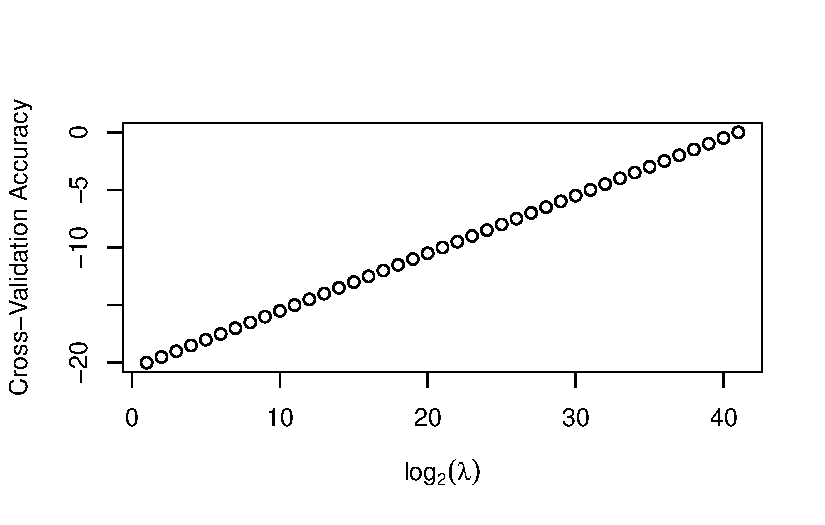
\includegraphics{hm4_files/figure-pdf/unnamed-chunk-23-1.pdf}

}

\end{figure}

\hypertarget{during-the-log2lamda-value-increase-the-cv-accuracy-also-increase}{%
\section{during the log2(lamda) value increase ,the cv accuracy also
increase}\label{during-the-log2lamda-value-increase-the-cv-accuracy-also-increase}}

\begin{center}\rule{0.5\linewidth}{0.5pt}\end{center}

3.5 (25 points)

First, use the \texttt{model.matrix()} function to convert the
covariates of \texttt{df} to a matrix format

\begin{Shaded}
\begin{Highlighting}[]
\NormalTok{covariate\_matrix }\OtherTok{\textless{}{-}} \FunctionTok{model.matrix}\NormalTok{(full\_model)[, }\SpecialCharTok{{-}}\DecValTok{1}\NormalTok{]}
\FunctionTok{head}\NormalTok{(covariate\_matrix)}
\end{Highlighting}
\end{Shaded}

\begin{verbatim}
  pclass sexmale age    fare siblings parents
1      3       1  22  7.2500        1       0
2      1       0  38 71.2833        1       0
3      3       0  26  7.9250        0       0
4      1       0  35 53.1000        1       0
5      3       1  35  8.0500        0       0
6      3       1  27  8.4583        0       0
\end{verbatim}

Now, initialize the covariates \(X\) and the response \(y\) as
\texttt{torch} tensors

\begin{Shaded}
\begin{Highlighting}[]
\NormalTok{X }\OtherTok{\textless{}{-}} \FunctionTok{torch\_tensor}\NormalTok{(covariate\_matrix, }\AttributeTok{dtype =} \FunctionTok{torch\_float32}\NormalTok{()) }\CommentTok{\# Insert your code here}
\NormalTok{y }\OtherTok{\textless{}{-}} \FunctionTok{torch\_tensor}\NormalTok{(titanic\_data}\SpecialCharTok{$}\NormalTok{y, }\AttributeTok{dtype =} \FunctionTok{torch\_float32}\NormalTok{()) }\CommentTok{\# Insert your code here}
\end{Highlighting}
\end{Shaded}

Using the \texttt{torch} library, initialize an \texttt{nn\_module}
which performs logistic regression for this dataset. (Remember that we
have 6 different covariates)

\begin{Shaded}
\begin{Highlighting}[]
\NormalTok{logistic }\OtherTok{\textless{}{-}} \FunctionTok{nn\_module}\NormalTok{(}
  \AttributeTok{initialize =} \ControlFlowTok{function}\NormalTok{() \{}
\NormalTok{    self}\SpecialCharTok{$}\NormalTok{f }\OtherTok{\textless{}{-}} \FunctionTok{nn\_linear}\NormalTok{(}\AttributeTok{in\_features =} \DecValTok{6}\NormalTok{, }\AttributeTok{out\_features =} \DecValTok{1}\NormalTok{) }\CommentTok{\# Insert your code here}
\NormalTok{    self}\SpecialCharTok{$}\NormalTok{g }\OtherTok{\textless{}{-}} \FunctionTok{nn\_dropout}\NormalTok{(}\AttributeTok{p =} \FloatTok{0.5}\NormalTok{) }\CommentTok{\# Insert your code here}
\NormalTok{  \},}
  \AttributeTok{forward =} \ControlFlowTok{function}\NormalTok{(x) \{}
\NormalTok{    x }\OtherTok{\textless{}{-}}\NormalTok{ self}\SpecialCharTok{$}\FunctionTok{f}\NormalTok{(x)}
\NormalTok{    x }\OtherTok{\textless{}{-}}\NormalTok{ self}\SpecialCharTok{$}\FunctionTok{g}\NormalTok{(x)}
    \FunctionTok{torch\_sigmoid}\NormalTok{(x) }\CommentTok{\# Insert your code here}
\NormalTok{  \}}
\NormalTok{)}

\NormalTok{f }\OtherTok{\textless{}{-}} \FunctionTok{logistic}\NormalTok{()}
\end{Highlighting}
\end{Shaded}

You can verify that your code is right by checking that the output to
the following code is a vector of probabilities:

\begin{Shaded}
\begin{Highlighting}[]
\FunctionTok{head}\NormalTok{(}\FunctionTok{f}\NormalTok{(X))}
\end{Highlighting}
\end{Shaded}

\begin{verbatim}
torch_tensor
 0.1982
 1.0000
 0.5000
 0.5000
 0.5000
 0.5000
[ CPUFloatType{6,1} ][ grad_fn = <SliceBackward0> ]
\end{verbatim}

Now, define the loss function \texttt{Loss()} which takes in two tensors
\texttt{X} and \texttt{y} and a function \texttt{Fun}, and outputs the
\textbf{Binary cross Entropy loss} between \texttt{Fun(X)} and
\texttt{y}.

\begin{Shaded}
\begin{Highlighting}[]
\NormalTok{Loss }\OtherTok{\textless{}{-}} \ControlFlowTok{function}\NormalTok{(X, y, Fun)\{}
\NormalTok{  predictions }\OtherTok{\textless{}{-}} \FunctionTok{Fun}\NormalTok{(X)}
\NormalTok{  loss }\OtherTok{\textless{}{-}} \FunctionTok{nnf\_binary\_cross\_entropy}\NormalTok{(predictions, y)}
\NormalTok{  loss }\CommentTok{\# Insert our code here}
\NormalTok{\}}
\end{Highlighting}
\end{Shaded}

Initialize an optimizer using \texttt{optim\_adam()} and perform
\(n=1000\) steps of gradient descent in order to fit logistic regression
using \texttt{torch}.

\begin{Shaded}
\begin{Highlighting}[]
\NormalTok{model }\OtherTok{\textless{}{-}} \FunctionTok{logistic}\NormalTok{()}
\NormalTok{f }\OtherTok{\textless{}{-}} \FunctionTok{logistic}\NormalTok{()}
\NormalTok{optimizer }\OtherTok{\textless{}{-}} \FunctionTok{optim\_adam}\NormalTok{(model}\SpecialCharTok{$}\NormalTok{parameters, }\AttributeTok{lr =} \FloatTok{0.01}\NormalTok{) }\CommentTok{\# Insert your code here}

\NormalTok{n }\OtherTok{\textless{}{-}} \DecValTok{1000}
\ControlFlowTok{for}\NormalTok{ (i }\ControlFlowTok{in} \DecValTok{1}\SpecialCharTok{:}\NormalTok{n) \{}
\NormalTok{  optimizer}\SpecialCharTok{$}\FunctionTok{zero\_grad}\NormalTok{()}
\NormalTok{  loss }\OtherTok{\textless{}{-}} \FunctionTok{Loss}\NormalTok{(X, y, f}\SpecialCharTok{$}\NormalTok{forward)}
\NormalTok{  loss}\SpecialCharTok{$}\FunctionTok{backward}\NormalTok{()}
\NormalTok{  optimizer}\SpecialCharTok{$}\FunctionTok{step}\NormalTok{()}
  
  \ControlFlowTok{if}\NormalTok{ (i }\SpecialCharTok{\%\%} \DecValTok{100} \SpecialCharTok{==} \DecValTok{0}\NormalTok{) \{}
    \FunctionTok{cat}\NormalTok{(}\StringTok{"Iteration: "}\NormalTok{, i, }\StringTok{" Loss: "}\NormalTok{, loss}\SpecialCharTok{$}\FunctionTok{item}\NormalTok{(), }\StringTok{"}\SpecialCharTok{\textbackslash{}n}\StringTok{"}\NormalTok{)}
\NormalTok{  \}}
\NormalTok{\}  }\CommentTok{\# Insert your code for gradient descent here}
\end{Highlighting}
\end{Shaded}

\begin{verbatim}
Iteration:  100  Loss:  9.641179 
Iteration:  200  Loss:  8.754433 
Iteration:  300  Loss:  8.593785 
Iteration:  400  Loss:  9.358589 
Iteration:  500  Loss:  9.392714 
Iteration:  600  Loss:  9.541448 
Iteration:  700  Loss:  9.58147 
Iteration:  800  Loss:  9.138812 
Iteration:  900  Loss:  9.444464 
Iteration:  1000  Loss:  10.10792 
\end{verbatim}

Using the final, optimized parameters of \texttt{f}, compute the compute
the predicted results on \texttt{X}

\begin{Shaded}
\begin{Highlighting}[]
\NormalTok{predicted\_probabilities }\OtherTok{\textless{}{-}} \FunctionTok{f}\NormalTok{(X) }\SpecialCharTok{\%\textgreater{}\%} \FunctionTok{as\_array}\NormalTok{()}
\NormalTok{torch\_predictions }\OtherTok{\textless{}{-}} \FunctionTok{ifelse}\NormalTok{(predicted\_probabilities }\SpecialCharTok{\textgreater{}} \FloatTok{0.5}\NormalTok{, }\DecValTok{1}\NormalTok{, }\DecValTok{0}\NormalTok{) }\CommentTok{\# Insert your code here}

\FunctionTok{overview}\NormalTok{(torch\_predictions, titanic\_data}\SpecialCharTok{$}\NormalTok{y)}
\end{Highlighting}
\end{Shaded}

\begin{verbatim}
   accuracy     error false_positive_rate false_negative_rate
1 0.6144307 0.3855693                   0           0.3855693
\end{verbatim}

\begin{center}\rule{0.5\linewidth}{0.5pt}\end{center}

3.6 (5 points)

Create a summary table of the \texttt{overview()} summary statistics for
each of the \(4\) models we have looked at in this assignment, and
comment on their relative strengths and drawbacks.

\begin{Shaded}
\begin{Highlighting}[]
\NormalTok{models }\OtherTok{\textless{}{-}} \FunctionTok{list}\NormalTok{(step\_model)}

\NormalTok{results }\OtherTok{\textless{}{-}} \FunctionTok{lapply}\NormalTok{(models, }\ControlFlowTok{function}\NormalTok{(model) \{}
\NormalTok{  predicted }\OtherTok{\textless{}{-}} \FunctionTok{predict}\NormalTok{(model, }\AttributeTok{type =} \StringTok{"response"}\NormalTok{) }\SpecialCharTok{\textgreater{}} \FloatTok{0.5}
  \FunctionTok{overview}\NormalTok{(predicted, titanic\_data}\SpecialCharTok{$}\NormalTok{y)}
\NormalTok{\})}


\NormalTok{summary\_table }\OtherTok{\textless{}{-}} \FunctionTok{do.call}\NormalTok{(rbind, results)}
\NormalTok{summary\_table}
\end{Highlighting}
\end{Shaded}

\begin{verbatim}
   accuracy     error false_positive_rate false_negative_rate
1 0.7959414 0.2040586          0.08568207           0.1183766
\end{verbatim}

\pagebreak

\begin{center}\rule{0.5\linewidth}{0.5pt}\end{center}

\begin{tcolorbox}[enhanced jigsaw, leftrule=.75mm, left=2mm, coltitle=black, rightrule=.15mm, titlerule=0mm, colbacktitle=quarto-callout-note-color!10!white, toprule=.15mm, bottomrule=.15mm, opacityback=0, arc=.35mm, colframe=quarto-callout-note-color-frame, title=\textcolor{quarto-callout-note-color}{\faInfo}\hspace{0.5em}{Session Information}, opacitybacktitle=0.6, toptitle=1mm, breakable, bottomtitle=1mm, colback=white]

Print your \texttt{R} session information using the following command

\begin{Shaded}
\begin{Highlighting}[]
\FunctionTok{sessionInfo}\NormalTok{()}
\end{Highlighting}
\end{Shaded}

\begin{verbatim}
R version 4.3.2 (2023-10-31 ucrt)
Platform: x86_64-w64-mingw32/x64 (64-bit)
Running under: Windows 11 x64 (build 22631)

Matrix products: default


locale:
[1] LC_COLLATE=English_United States.utf8 
[2] LC_CTYPE=English_United States.utf8   
[3] LC_MONETARY=English_United States.utf8
[4] LC_NUMERIC=C                          
[5] LC_TIME=English_United States.utf8    

time zone: America/New_York
tzcode source: internal

attached base packages:
[1] stats     graphics  grDevices utils     datasets  methods   base     

other attached packages:
 [1] pracma_2.4.4   broom_1.0.5    nnet_7.3-19    torch_0.12.0   caret_6.0-94  
 [6] lattice_0.21-9 ggplot2_3.4.4  car_3.1-2      carData_3.0-5  corrplot_0.92 
[11] stringr_1.5.1  purrr_1.0.2    tidyr_1.3.1    readr_2.1.5    dplyr_1.1.4   

loaded via a namespace (and not attached):
 [1] tidyselect_1.2.0     timeDate_4032.109    fastmap_1.1.1       
 [4] pROC_1.18.5          digest_0.6.34        rpart_4.1.21        
 [7] timechange_0.3.0     lifecycle_1.0.4      survival_3.5-7      
[10] processx_3.8.3       magrittr_2.0.3       compiler_4.3.2      
[13] rlang_1.1.3          tools_4.3.2          utf8_1.2.4          
[16] yaml_2.3.8           data.table_1.15.0    knitr_1.45          
[19] curl_5.2.0           bit_4.0.5            plyr_1.8.9          
[22] abind_1.4-5          withr_3.0.0          grid_4.3.2          
[25] stats4_4.3.2         fansi_1.0.6          colorspace_2.1-0    
[28] future_1.33.1        globals_0.16.3       scales_1.3.0        
[31] iterators_1.0.14     MASS_7.3-60          cli_3.6.2           
[34] crayon_1.5.2         rmarkdown_2.25       generics_0.1.3      
[37] rstudioapi_0.15.0    future.apply_1.11.1  reshape2_1.4.4      
[40] tzdb_0.4.0           splines_4.3.2        parallel_4.3.2      
[43] coro_1.0.4           vctrs_0.6.5          glmnet_4.1-8        
[46] hardhat_1.3.1        Matrix_1.6-1.1       jsonlite_1.8.8      
[49] callr_3.7.3          hms_1.1.3            bit64_4.0.5         
[52] listenv_0.9.1        foreach_1.5.2        gower_1.0.1         
[55] recipes_1.0.10       glue_1.7.0           parallelly_1.37.1   
[58] codetools_0.2-19     ps_1.7.6             shape_1.4.6         
[61] lubridate_1.9.3      stringi_1.8.3        gtable_0.3.4        
[64] munsell_0.5.0        tibble_3.2.1         pillar_1.9.0        
[67] htmltools_0.5.7      ipred_0.9-14         lava_1.8.0          
[70] R6_2.5.1             vroom_1.6.5          evaluate_0.23       
[73] backports_1.4.1      class_7.3-22         Rcpp_1.0.12         
[76] nlme_3.1-163         prodlim_2023.08.28   xfun_0.41           
[79] pkgconfig_2.0.3      ModelMetrics_1.2.2.2
\end{verbatim}

\end{tcolorbox}



\end{document}
